\documentclass[12pt]{article}

% Packages
\usepackage{amsmath}
\usepackage{graphicx}
\usepackage[margin=0.5in, footskip=0.1in]{geometry}
\usepackage{multicol}
\usepackage{enumitem} % For itemize spacing control
\usepackage{titlesec} % For sections spacing control
\usepackage{xspace}

\begin{document}
\newgeometry{top=1in, left=0.5in, right=0.5in, bottom=0.5in, footskip=0.1in}
   \begin{center}
    \vspace{1.5cm}
    \vfill
       \Huge
       \textbf{CIFAR-10 Classification Coursework}

       \vspace{0.5cm}
       \LARGE
       ECS6P9U - Neural Networks and Deep Learning
        
       \large
       \vspace{0.5cm}
       \textbf{Christian Juresh} - 210517307
       \vspace{1.5cm}
   \end{center}

\section{Dataset and Dataloaders: 5\%}

Two sets of transformations are defined. One is for dataset augmentation: used for the training dataset, and one for standard processing: used for the validation and testing datasets. To prevent overfitting, the dataset augmentation transformation includes several steps to artificially increase the diversity of the training data:

\begin{itemize}
\item \textbf{RandomHorizontalFlip:} Mirrors images horizontally at random.

\item \textbf{RandomCrop:} Randomly crops the images and adds padding.

\item \textbf{ToTensor:} Converts the images to PyTorch tensors.

\item \textbf{Cutout:} Uses my custom implementation of a random masking technique that "cuts out" one or more rectangular patches from the input image. 

\item \textbf{Normalize:} Standardises the colors of the images.
\end{itemize}
The testing dataset is a batch size of 4, and only includes the ToTensor and Normalize transformations. This is so that the model is tested on the original images for accurate results. A batch size of 64 for training gives a balance of speed and accuracy.

\section{Model: 40\%}
\subsection{Block}
The \texttt{Block} class represents one instance of many blocks, which are responsible for a sequence of operations that map an input tensor to a transformed output. It uses an \texttt{AdaptiveAvgPool2d} layer to perform spatial averaging, reducing each channel to a vector of \(d\). This vector is then transformed by a \texttt{Linear} layer, which outputs a vector \( a \) of length \( K \), the number of convolutional layers, where each element is a weight. The convolutional layers consist of a \texttt{Conv2d} layer, batch normalization, and a non-linear \texttt{ReLU} activation function. In the forward pass, a weight vector \( a \) is calculated from the linear layer's output, softmax is applied to obtain a distribution of weights, and the outputs of the convolutional layers are combined based on these weights to produce a single tensor \( O \). 

\restoregeometry
\subsection{Backbone}
The \texttt{Backbone} class is responsible for constructing \( N \) Blocks. It does this by sequentially stacking multiple different stages of Block instances in two \texttt{for} loops.  

\subsection{Classifier}
The \texttt{Classifier} class creates a classifier that takes the output from the final Block in the Backbone and computes a mean feature vector by applying a SpatialAveragePool. This mean feature vector is then passed to a multi-layer perceptron (MLP) classifier, consisting of one fully connected layer, \texttt{ReLU} activation, dropout for regularization, and then another fully connected layer.

\subsection{Model}
The \texttt{Model} class combines the Backbone and Classifier to create a Convolutional Neural Network (CNN). The forward pass puts tensor \( X \) through the Backbone, receives the \( O_N \) output from the \( N_{\text{th}} \) Block, and then puts it through the Classifier. 

\section{Loss and Optimizer: 5\%}
\texttt{CrossEntropyLoss} is used as the loss function. It applies a softmax function to the output of the network to compute probabilities, and then calculates the loss between the predicted probabilities and the true class labels. \texttt{optim.SGD} is used as a Stochastic Gradient Descent optimiser, which updates the weights of the model based on the gradient of the loss function with respect to the weights. It finds the set of weights that minimise the loss function. Learning rate controls how much the weights are adjusted by, and momentum accelerates the optimiser in the right direction. Weight decay helps in preventing overfitting by penalising large weights. \texttt{lr\_scheduler.CosineAnnealingLR} is used to adjust the learning rate following a cosine annealing schedule. It reduces the learning rate between an upper and lower boundary over the number of epochs. This improves performance and allows the model to find better local minima.

\section{Training Script: 30\%}
\subsection{Training Loop}
The training loop simply runs the training function over a set number of epochs.\texttt{lr\_scheduler.step} is called to adjust the learning rate at the end of each epoch.

\subsubsection{Function \texttt{train\_epoch}}
The \texttt{train\_epoch} function begins by setting the model to training mode. It iterates through the \textit{loader}, which provides batches of \textit{inputs} and their \textit{labels}. The data is then moved to the correct device.\\ \texttt{optimizer.zero\_grad} clears any old gradients from the last step so that they don't accumulate. Then the model computes the prediction for the input data. \texttt{criterion} calculates the difference between the model's predictions and the actual labels, and produces a scalar value to represent the model's performance. \texttt{loss.backward} computes the gradient of the loss with respect to the model's parameters, which are then used to adjust and update the weights with \texttt{optimizer.step}

\newpage
\subsection{Hyperparameters}
\vspace{-0.3cm}
% Reduce space around sections
\titlespacing*{\subsubsection}{0pt}{3ex plus 1ex minus .2ex}{1ex plus .2ex}

% Tighten spacing for itemize
\setlist[itemize]{topsep=0pt, partopsep=0pt, parsep=0pt, itemsep=1pt}

\begin{multicols}{2}
\subsubsection*{Dataset Augmentation Transformation}

\begin{itemize}
  \item \texttt{RandomHorizontalFlip}
    \begin{itemize}
      \item \texttt{Probability} = 0.5
    \end{itemize}
  \item \texttt{RandomCrop}
    \begin{itemize}
      \item \texttt{Size} = 32
      \item \texttt{Padding} = 4
    \end{itemize}
  \item \texttt{Cutout}
    \begin{itemize}
      \item \texttt{Number of holes} = 1
      \item \texttt{Length of each hole} = 16
    \end{itemize}
  \item \texttt{Normalize}
    \begin{itemize}
      \item \texttt{Mean \& SD} = $(0.5, 0.5, 0.5)$
    \end{itemize}
\end{itemize}

\subsubsection*{Dataset Loading}
\begin{itemize}
    \item \texttt{training batch size} = 128
    \item \texttt{vallidation batch size} = 4
\end{itemize}

\subsubsection*{Model Architecture}
\begin{itemize}
    \item \texttt{number of classes} = 10
    \item \texttt{input channels} = 3 (RGB)
\end{itemize}

\vspace{0.3cm}

\begin{itemize}
    \item \texttt{convolutions} = 2
    \item \texttt{layer output channels} = [64, 128, 256, 512]
    \item \texttt{blocks} = [2, 2, 2, 2]
\end{itemize}

\subsubsection*{Training}
\begin{itemize}
    \item \texttt{epochs} = 150
\end{itemize}

\subsubsection*{Optimisers}
\begin{itemize}
    \item \texttt{learning rate} = 0.2
    \item \texttt{momentum} = 0.9
    \item \texttt{weight decay} = $5 \times 10^{-4}$
\end{itemize}
\end{multicols}

\fontsize{12}{12}\selectfont
\subsection{Plot}
\vspace{-0.5cm}
\begin{center}
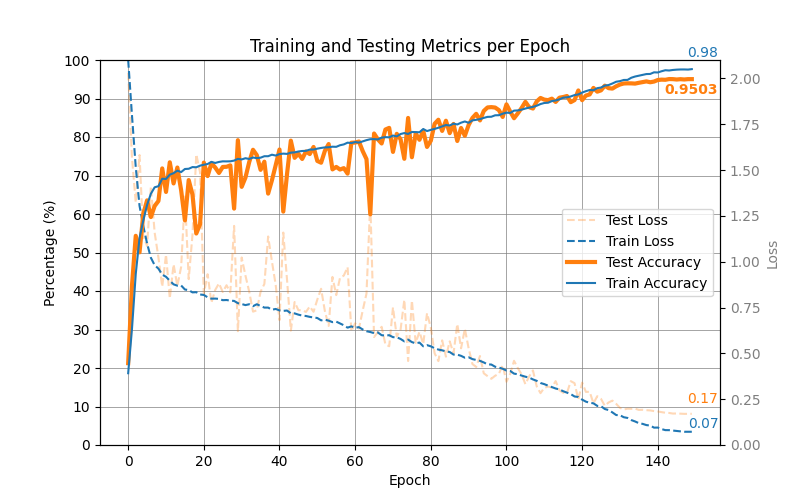
\includegraphics[width=\textwidth]{metrics.png}
\end{center}

\vspace{-0.5cm}
\section{Final Model Accuracy: 20\%}
Final model accuracy: 95.03\%

\end{document}